\chapter{Pendahuluan}
\section{Sejarah singkat}
Python dibangun oleh Guido van Rossum (\figurename~\ref{fig:guido}\footnote{\url{https://gvanrossum.github.io/images/guido-headshot-2019.jpg}}) pada sekitar tahun 1980 di \textit{Centrum Wiskunde \& Informatica} (CWI) di Belanda\cite{python3intro}. Nama Python diambil dari program TV favorit Guido yang berjudul '''Monty Pythons Flying Circus''' yang tayang pada kisaran tahun 1969-1974.

\begin{figure}
  \begin{center}
    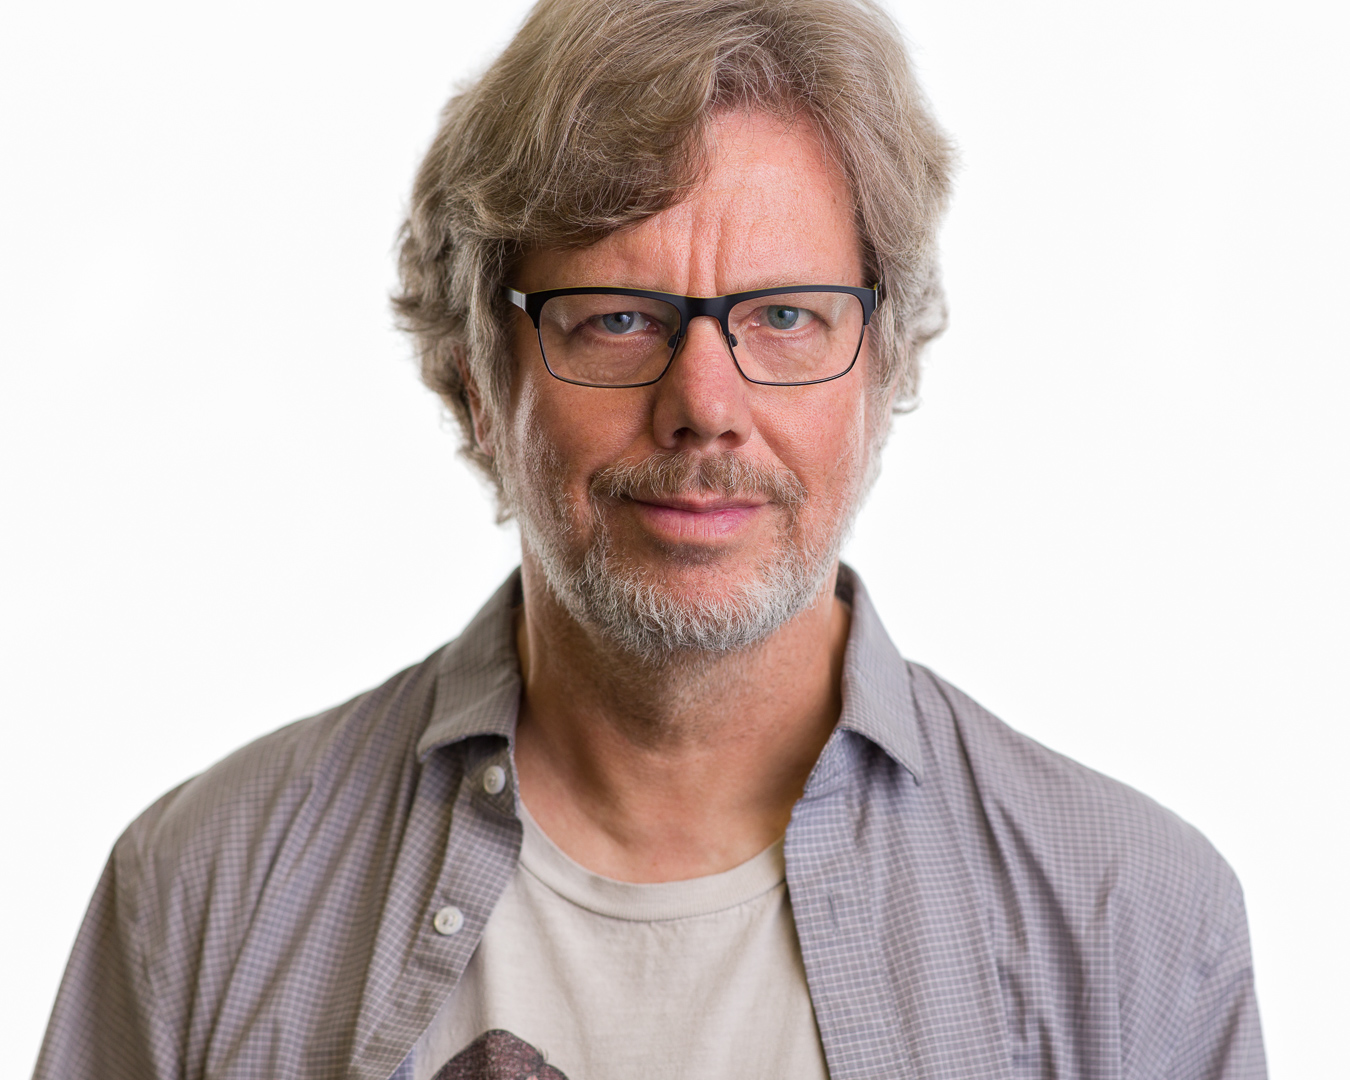
\includegraphics[scale=.5]{pics/guido-headshot-2019.jpg}
    \caption{Guido van Rossum}
    \label{fig:guido}
  \end{center}
\end{figure}

\section{Kenapa Python?}
Berikut adalah beberapa jawaban dari pertanyaan tersebut.
\begin{itemize}
  \item \textit{Multiplatform}. Python adalah bahasa pemrograman yang tersedia pada sejumlah \textit{platform} sistem operasi seperti \texttt{GNU Linux, Windows dan Mac}. Selain itu, Python juga tersedia pada \textit{platform} perangkat bergerak seperti Android dan \textit{embedded system}\footnote{\url{https://wiki.python.org/moin/EmbeddedPython}}.
  \item Mudah. Python merupakan bahasa pemrograman yang mudah karena \texttt{syntax} yang sederhana, sehingga mudah dikuasai bahkan oleh pengguna yang tidak memiliki latar belakang pendidikan formal di bidang ilmu komputer.
  \item Pustaka. Pustaka pendukung untuk banyak bidang ilmu tersedia secara bebas (bahkan terawat dengan baik oleh komunitas), terutama dalam bidang pembelajaran mesin di mana Python sangat populer saat ini.
\end{itemize}
